%%%%%%%%%%%%%%%%%%%%%%%%%%%%%%%%%%%%%%%%%%%%%%%%%%%%%%%%%%%
% LaTeX Template ~ 'tau-book.tex'
% Version 2.1 (04/03/2024)
%
% Description: 
% Tau-book is a LaTeX template that offers a clean and 
% professional design for lab reports or academic papers.
% The clarity of the code structure makes it easy to 
% understand and modify for your needs. This template uses 
% an easy-to-read font and high quality equations with "stix2".
%
% Author: 
% Guillermo Jimenez (memo.notess1@gmail.com)
% 
% License:
% Creative Commons CC BY 4.0
%%%%%%%%%%%%%%%%%%%%%%%%%%%%%%%%%%%%%%%%%%%%%%%%%%%%%%%%%%%
% You may modify 'tau-book.cls' file according to your
% needs and preferences. This LaTeX class file defines 
% the document layout, formatting, and behavior.
%%%%%%%%%%%%%%%%%%%%%%%%%%%%%%%%%%%%%%%%%%%%%%%%%%%%%%%%%%%
%     BIBLIOGRAPHY WITH BIBLATEX IN EXTERNAL EDITORS:
% If the bibliography does not show up, try running the 
% 'tau-book.cls' and 'tau.bib' file with biber from the 
% MikTeX console or your preferred LaTeX distribution to 
% generate the .aux files and (re)run tau-book.tex again.
%%%%%%%%%%%%%%%%%%%%%%%%%%%%%%%%%%%%%%%%%%%%%%%%%%%%%%%%%%%
%                          WARNING:
% It is important to proceed with caution and ensure that 
% any modifications made are compatible with LaTeX 
% syntax and conventions to avoid errors or unexpected 
% behavior in the document compilation process.
%%%%%%%%%%%%%%%%%%%%%%%%%%%%%%%%%%%%%%%%%%%%%%%%%%%%%%%%%%%

\documentclass[11pt,a4paper,twoside]{tau-book}
\usepackage[english]{babel}
\usepackage{tau}
\usepackage{mathtools}
\usepackage{float}


%----------------------------------------------------------
% Title
%----------------------------------------------------------

\title{Caffeine and Timed Up and Go Cognitive Test}

%----------------------------------------------------------
% Authors, affiliations and professor
%----------------------------------------------------------


\author[a,c]{\small Oliver Siu}
\author[a,c,d]{Nicholas Cassol-Pawson}
\author[a,b,c]{Emma Vidal}
\author[a,c]{Romy Guo}
\author[a,b,c]{Kanzah Jamil}
\author[a,c]{Max Chalekson}
\author[a,c,d]{Jesper White}




%----------------------------------------------------------

\affil[a]{University of California, Los Angeles (UCLA)}
\affil[b]{Department of Mathematics}
\affil[c]{Department of Statistics \& Data Science}
\affil[d]{Department of Economics}


\professor{Group 4 | S24-LEC2-STATS 101B: Introduction to Design and Analysis of Experiment | Dr. Maria Cha}



%----------------------------------------------------------
% Footpage notes
%----------------------------------------------------------

\institution{UCLA}
\ftitle{Caffeine and Timed Up and Go Cognitive Test}
\theday{June 9, 2024} % \today
\etal{Group 4}
\course{STATS 101B: Introduction to Design and Analysis of Experiment}

%----------------------------------------------------------
% Abstract
%----------------------------------------------------------

%\theabstract{}

%----------------------------------------------------------

%\keywords{\LaTeX\ class, lab report, academic paper, tau-book class}

%----------------------------------------------------------

\begin{document}
	
    \maketitle
    %\abscontent
    % \tableofcontents  % Uncomment to activate the table of contents
    \thispagestyle{firststyle}

%----------------------------------------------------------
% The document begins
%----------------------------------------------------------


\section{Introduction}
    \taustart{C}affeine is one of the most widely consumed drugs worldwide, known for its stimulating effects on the central nervous system. It is commonly believed that caffeine enhances mental performance and physical energy, making it a popular choice in various consumer products, but research shows mixed evidence of caffeine’s performance-boosting capabilities. Caffeine has varying effects on different individuals and may not always improve mental capabilities such as attention \cite{Anderson2000} (Anderson, 2000, p. 18). Depending on the task, caffeine may or may not improve mental performance \cite{Stepan2021} (Stephan et al., 2021, p. 1381).
    
    Verifying the exact benefits and limitations of caffeine remains under study and is important for determining when caffeine consumption is most appropriate and effective.
    
    \subsection{Approach}
    Previous research suggests that caffeine may improve general alertness but does not have a pronounced effect on performance when it comes to more complicated and demanding tasks. So, we expect caffeine to improve performance when carrying out light physical and mental tasks. 
    
    To test this hypothesis, we used a Timed Up and Go Cognitive test to assess coordination and mental performance in working-age adults (between the ages of 20 and 65). We wished to see if taking caffeine could improve their performance in tasks that demand physical abilities and mental focus. 
    
    The Timed Up and Go Cognitive test seems perfect for this: it asks participants to rise from a chair, walk 3 meters, turn around, walk back to the chair, and sit down, all while counting backward by 3 from 72, which targets both their ability to concentrate on a somewhat complex mental task and their general coordination. Participants’ times for completion are recorded in seconds, and a faster time indicates better performance. Tests were administered at 2:00 p.m. on a Monday, and subjects were chosen from the Islands Project, a population of virtual human subjects created by Dr. Michael Bulmer at the University of Queensland. Informed consent was obtained from all participants.

\section{Methods}

\subsection{Design of Experiment}
During our preliminary design of the experiment, we were concerned about two separate situations: the climate of the subjects’ home islands impacting the rate of the caffeine intake of the subjects and the age of the subjects causing them to have different baseline scores on the tests and intake caffeine in different manners. We opted to block over these two variables. 

There are three islands and we defined three age groups of 15 years each: 20-34, 35-49, and 50-65. Since we had two blocked factors of 3 levels each, we chose to run a replicated Latin square design. This meant that we would need three levels for our caffeine dosage. We chose to run the experiment with dosage levels 0, 100, and 200 mg of caffeine. 

Since there are two blocking factors at three levels each, each replicate required nine runs of the experiment. We chose to do seven replicates of the experiment, so we generated seven random $3\times3$ Latin square designs. Our data and copies of the Latin squares are included in the Appendix \ref{appendix}. 

\subsection{Sampling}
We then randomly selected our subjects. Since we were blocking by island, we first randomly chose a village within the current island block with a random number generator. Then, within the village, we randomly selected a house and, if that house had a subject in the age category under investigation, we would ask them for consent to participate in the study. If there were multiple people who fell within the correct age bracket, we would randomly choose one of them. If we were denied consent, we would resample the house in the village until we got consent from someone in the age bracket. 

This sampling technique is a limitation of our experimental design, as it is not simple random sampling. Since each village has a different number of people, people living in smaller villages have a higher probability of being drawn. This is an inherent limitation of the island system, as there was no centralized roster of people on the island from which to draw the blocked sample.

\subsection{Sample Size and Power of the Test}

\begin{figure}[H]
        \raggedleft
        \begin{verbatim}
        Balanced one-way analysis
        of variance power calculation
        
        k = 3
        n = 21
        f = 0.3133475
        sig.level = 0.05
        power = 0.5751066
        
        NOTE: n is number in each group    
        \end{verbatim}
        \caption{R Output of Power}
        \label{fig:power_cognitive}
\end{figure}

After our experiment, we had data to calculate the power of our test (Figure \ref{fig:power_cognitive}). We computed an effect size of $f=0.313$ by finding the difference between the largest and smallest sample means, which is the largest difference in them, by definition. We then estimated the standard deviation with the standard error, which we computed by taking the square root of the mean square error, giving a value of $\widehat{\sigma} = 0.532$. Plugging all of these numbers into \texttt{pwr.text} in R, we found that a sample size of $n=63$ gives a power of $\approx$ 0.58. This is not satisfactory as it means that there is a $1-\text{power} = \beta = 42\%$ chance of accepting a false null hypothesis (making a Type II error).


\begin{figure}[H]
        \raggedleft
        \begin{verbatim}
        Balanced one-way analysis
        of variance power calculation
        
        k = 3
        n = 33.72766
        f = 0.3133475
        sig.level = 0.05
        power = 0.8
        
        NOTE: n is number in each group    
        \end{verbatim}
        \caption{R Output of Recommended Observations}
        \label{fig:power_cognitive_2}
\end{figure}

An optimal test power would be around 80\%. To detect a maximum difference in mean test times of $f=0.313$ seconds, we calculated a suggested $n=33.7$ which recommends $n=34$ (Figure \ref{fig:power_cognitive_2}). Given $n=34$ observations per $k=3$ treatment groups, a sample size of $N=102$ is recommended.

\subsection{Model and Hypotheses}

The population model is 

$$
    y_{ijk} = \mu + \alpha_{i(l)} + \tau_{j} + \beta_{k(l)} + \rho_{l} + \epsilon_{ijkl}
$$


for $i, j, k \in 1, 2, 3$ and $l \in 1, 2, ..., 7$

\begin{itemize}
    \item $y_{ijk}$ is the change in time to complete the Timed Up and Go Cognitive test for the $i^{\text{th}}$ island and $k^{\text{th}}$ age group for the $j^{\text{th}}$ caffeine treatment;
    \item $\mu$ is the average difference in time to complete the cognitive test across all observations, before and after the caffeine intervention;
    \item $\alpha_{i(l)}$ is the $j^{\text{th}}$ island block effect within replicate $l$;
    \item $\tau_{j}$ j is the $j^{\text{th}}$ caffeine effect;
    \item $\beta_{k(l)}$ is the $k^{\text{th}}$ age block effect within replicate $l$;
    \item $\rho_{l}$ is the $l^{\text{th}}$ replicate effect; and
    \item $\epsilon_{ijkl}$ is the random error

\end{itemize}

The objective is to assess the impact of different dosages of caffeine on the Timed Up and Go Cognitive test scores of individuals blocked by their age groups and geographic locations.

Therefore, we wish to test the hypotheses:
\begin{align*}
    &H_0: \tau_1 = \tau_2 = \tau_3 = 0 \\
    &H_1: \tau_j \ne 0, \text{at least one } j
\end{align*}


\section{Results and Interpretation}


\subsection{ANOVA Results}



\begin{figure}[H]
        \centering
        \begin{verbatim}
                        Df  Sum Sq  Mean Sq  
        factor(caffeine) 2   0.341   0.1706  
        factor(age)      2   0.748   0.3740    
        factor(island)   2   0.177   0.0883  
        factor(user)     6   1.113   0.1855   
        Residuals        50  14.145  0.2829
        
                            F value Pr(>F)
        factor(caffeine)    0.603    0.551
        factor(age)         1.322    0.276
        factor(island)      0.312    0.733
        factor(user)        0.656    0.685
        Residuals
        \end{verbatim}
        \caption{R output of ANOVA}
        \label{fig:cognitive}
\end{figure}
Figure \ref{fig:cognitive} shows $p = 0.551 > \alpha = 0.05$, so we fail to reject the null hypothesis at a 5\% significance level. This suggests that caffeine does not significantly influence this measure of cognitive performance.

\subsection{Diagnostic Plots}
\begin{figure}[H]
        \centering
        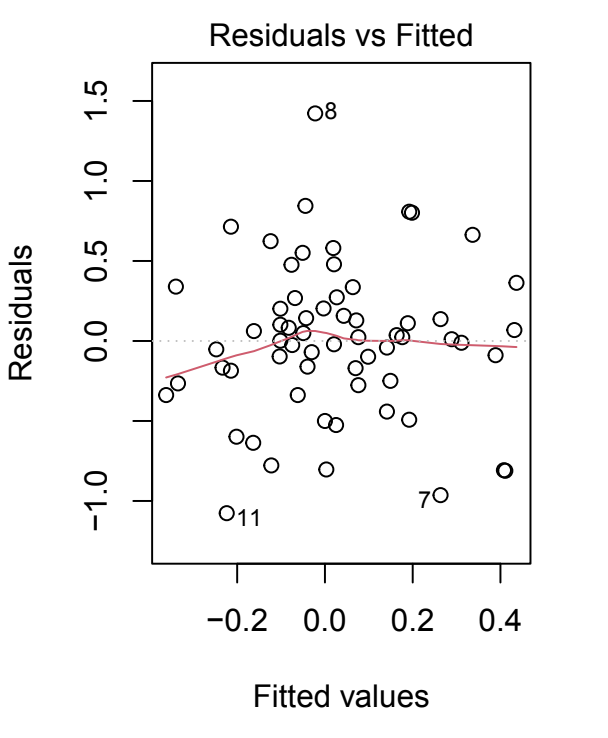
\includegraphics[width=0.8\columnwidth]{Figures/diagnostic_fitted.png}
        \caption{Residuals vs. Fitted Diagnostic Plot}
        \label{fig:diagnostic_fitted}
\end{figure}

In Figure \ref{fig:diagnostic_fitted}, the Residuals vs. Fitted Values plot shows no obvious patterns, and the scattering along the horizontal axis is similar to the scattering along the vertical axis, indicating homoskedasticity, i.e., the constant variance assumption is satisfied.

\begin{figure}[H]
        \centering
        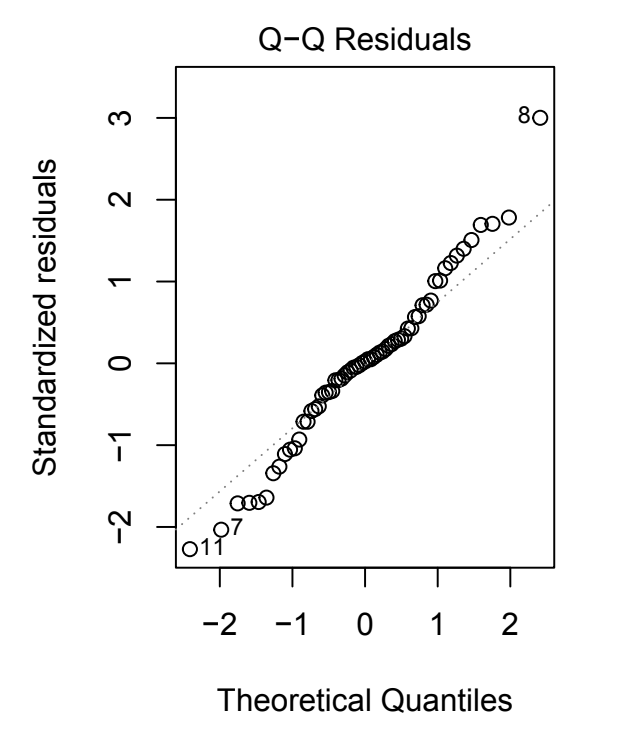
\includegraphics[width=0.8\columnwidth]{Figures/diagnostic_qq.png}
        \caption{Normal Q-Q Diagnostic Plot}
        \label{fig:diagnostic_qq}
\end{figure}

In the normal Q-Q plots for the residuals (Figure \ref{fig:diagnostic_qq}), the points lie approximately along the reference line, indicating that the residuals are normally distributed. 

Both of the diagnostic plots suggest that the assumptions of the model are reasonably met.

\subsection{Block Analysis}

\begin{figure}[H]
        \centering
        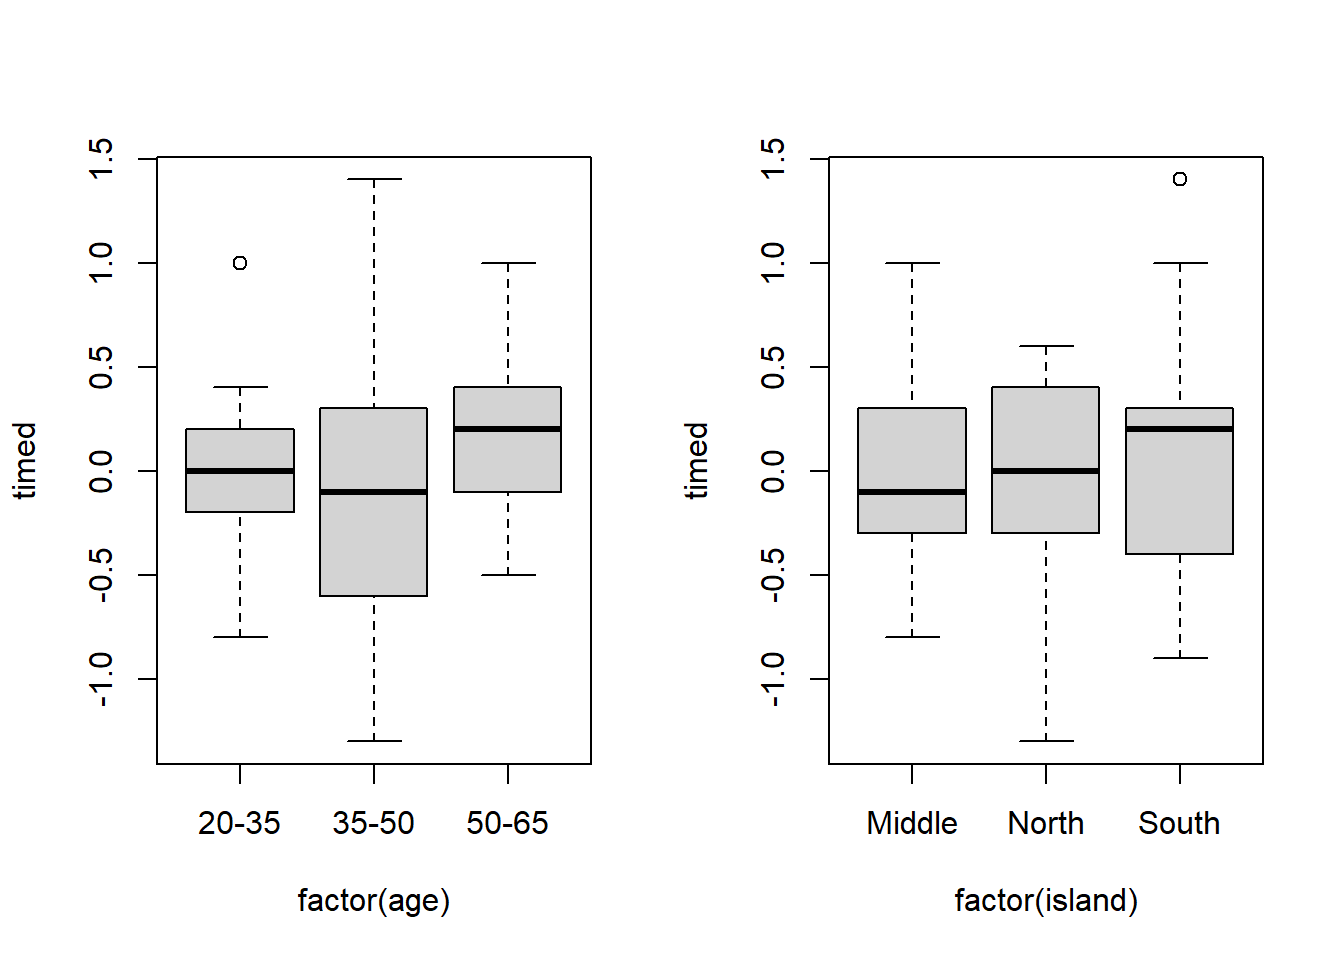
\includegraphics[width=1\columnwidth]{Figures/block_means_plot.png}
        \caption{Plots of Block Means}
        \label{fig:block_means_plot}
\end{figure}

The ANOVA results cannot be used to discuss the significance of the block effect, as the ANOVA process is not providing estimates for the blocking factors, rather it is considering them to be random variations. However, we can compare the mean values across the blocks to try to determine whether they were necessary. 

We plotted the mean values across the 3 blocks for age group and the 3 blocks for the islands in paired box plots. 

Looking at the age group results in Figure \ref{fig:block_means_plot}, we can see that the means are all very similar, with a range of 0.2: spanning from an average difference of -0.1 seconds in the 35-49 age group to 0.1 in the 50-65 age group. The total range of the observed differences is just under 3 seconds, with a minimum difference before and after the intervention in time to take the Timed Up and Go test of -1.4 and a maximum difference of 1.5. Since the mean range is only about 3\% of the total range of the times, controlling for age group likely did not have much impact on our final results, so pooling the data would have been fine. 

Similarly, we look at the island blocks in Figure \ref{fig:block_means_plot}. Here we see that there is a slightly larger range for the mean difference in time to take the Timed Up and Go test, with the highest average difference of 0.3 on the South island and the lowest average difference of -0.1 on the Middle island. This leads to a range of 0.4 seconds, just over one tenth of the total range of 3 seconds. This indicates that the island block probably also did not have much of an impact on the final results of our report. 

\subsection{Interpretation of Results}
Our results suggest that caffeine intake does not significantly affect the time to complete the Timed Up and Go Cognitive test. Despite the expectation that caffeine might enhance cognitive performance, our study found a $p$-value of 0.551 on this effect, indicating that we should accept the null hypothesis that there is no statistically significant effect of caffeine on the Timed Up and Go Cognitive coordination scores at a 5\% level. 

These findings highlight the complexity of factors that play into cognitive and motor skills and suggest that factors other than caffeine intake might play more important roles. Further research could explore different cognitive performance measures or consider other variables that might interact with caffeine consumption to affect cognitive outcomes. The diagnostic plots confirm that the ANOVA assumptions were met, which supports the validity of our findings.

\section{Discussion and Conclusion}
\subsection{Summary}
Our study focused on investigating the effects of caffeine on performance in light physical and mental tasks and allowed us to understand that caffeine products are not effective on cognition. To do this, we designed and tested subjects using a $3\times3$ Latin Square Design experiment, with caffeine dosages of 0 mg, 100 mg, or 200 mg of caffeine. We then tested their coordination and mental capabilities using the Timed Up and Go Cognitive test, both before and after administering the caffeine intervention.

In our analysis, we accounted for the variability introduced by island and age group by incorporating them as blocking factors. Our hypothesis sought to determine whether our treatment factor, caffeine dosage, had a significant effect on participants’ cognitive and coordination abilities. The findings for this experiment show that caffeine does not significantly influence the performance of the tasks completed among young and middle-aged adults at the 5\% significance level. This result challenges the belief that caffeine enhances cognitive performance and physical ability, requiring further investigation to fully understand the drug's effect on these parameters.

\subsection{Applying Our Results to the Real World}
This study utilizes the concept of optimizing the timing of caffeine consumption and its implications for an individual's cognitive and physical performance. Understanding such scenarios allows up to reap maximum benefits of this drug in real-world scenarios.

To start, considering the peak level of caffeine effectiveness occurs around the one-hour mark after consumption \cite{Liguori1997} (Liguori, 1997, p. 724), individuals can strategically time their caffeine intake to coincide with tasks that require heightened awareness and focus. By aligning caffeine consumption with the timing of a task that requires cognitive processing, individuals may capitalize on the alertness provided by caffeine, improving their performance on tasks that require one's attention and quick reaction-time.

With the benefits of caffeine, it is important to understand that the effect of caffeine varies amongst individuals, influenced by factors such as, but not limited to, genetics, tolerance levels, and sensitivity to the drug \cite{James2014} (James, 2014, p. 118). Therefore, customized approaches to caffeine consumption for each individual allows them to optimize the drug's benefits, while minimizing the adverse effects.

Our findings suggest caffeine's effect on cognitive performance may not be consistent across all tasks \cite{Anderson2000} (Anderson, 2000, p. 10), for complex tasks, it is deemed uncertain as to how caffeine directly aids in those tasks that have many integral parts. Thus, further research should be completed to uncover more of the effects of caffeine on different cognitive aspects, to allow individuals to make decisions on how to optimize their productivity.

Our findings reflect some real-world experiments. An experiment that looked at the effects of having either a 250 mg dose of caffeine or a placebo on a reaction test suggested that there was no significant impact of caffeine dosage in either direction on the participant's concentration \cite{Ruijter2000} (Ruijter, 2000, pg. 29). 

\subsection{Limitations and Future Work}
There were several limitations underlying our study that could have led to us not finding any significant causal relations between caffeine and mental performance. As we mentioned earlier, one of the main limitations is due to our sampling method. It was not simple random sampling, rather it involved choosing subjects randomly within blocks, which may have introduced experimental bias. We followed this technique as we were constrained by the Islands system’s lack of a centralized population census, making it difficult to implement SRS within blocks. Individuals from smaller villages had a higher probability of being included in our sample, which affected how representative our sample was of island population as a whole. 

We believe that there is a second limitation that arose from an inherent difficulty with the Islands system: that the Islanders may not be programmed for caffeine consumption to directly impact their performance in the Timed Up and Go test. This is entirely plausible: the block effects that we detected did not seem to be significant, although since we didn't test for this in a statistically significant manner, they may actually be. However, since the blocks had such a small effect, we are led to believe that regardless of which island or age group an Islander comes from, the amount of caffeine they consumed did not seem to affect their performance on the cognitive and motor skills test that we ran on them. This stands in contrast to the literature we reviewed when devising our original hypothesis, which indicated that we should detect an improvement in these skills with an increase in caffeine dosage. 

In the future, we can make a few adjustments to our experiment to try to detect some effect between caffeine consumption and mental and/or physical performance. 

We could try to conduct a stronger form of sampling for the blocks to ensure that our sample population was chosen by SRS. This could increase the significance of the effects that we are looking for. However, as we noted before, even in our imperfectly sampled model, it is unlikely that the blocks are actually meaningful. 

We could also try expanding our subject pool to cover a larger range of ages: our experiment only looked at adults in young and middle age. However, there is a chance that caffeine consumption actually has a statistically significant effect on the cognitive and motor skills of older adults or younger children, and just young and middle-aged adults are unaffected by it. 

% Since the sample size is the main problem, maybe this should be our primary limitiation?
A third limitation was our limited sample size. The experiment utilized a replicated Latin square design with each of our group members as a replicate. This restricted our sample size to $N=63$ which produced a test power below an adequate level. Optimally, the power of the test should be around 80\% which would require a sample size of $N=102$, as indicated in Figure \ref{fig:power_cognitive_2}. Due to time constraints, we were unable to increase the replicates or alter the experiment design to accommodate a larger sample size. Future tests should include more observations to increase test power and reduce the chance of making a Type II error. Since the block and replicate effects were not significant, a different design may also be recommended to increase the sample size to achieve optimal test power and improve the accuracy of future experiments.

Finally, we could try running different tests on our subjects than the Timed Up and Go Cognitive test. As we indicated before, there is literature that suggests that there may be an effect between caffeine consumption and mental and physical performance. It could be that the Timed Up and Go cognitive test is not ideal for this situation, but the Islands project offers a whole host of tests that can be run that seem to target the skills that we are testing for, including a variety of logic and focus tasks, many different forms of light and heavy exercise, and several coordination-targeted activities. 

\newpage

\printbibliography

% \newpage\hbox{}\thispagestyle{empty}
\newpage

\appendix \section{Appendix}\label{appendix}

\subsection{Data}
\href{https://docs.google.com/spreadsheets/d/15w2DWU1tjqDd9jpK0eBlqL89jGZZJeL1wOMOckCUdbw/edit?usp=sharing}{Here} is a Google Spreadsheet with the data we collected. This file was exported to a .csv to analyze the data in R.

\subsection{Latin Squares}
\begin{itemize}
    \item A, B, and C correspond to the 0 mg, 100 mg, and 200 mg caffeine treatments, respectively.
    \item The numbers after the equal correspond to the measured change in test score for Timed Up and Go Cognitive.
    \item The rows correspond to the age range blocks (20-34, 35-49, and 50-65).
    \item The columns correspond to the island block (Ironbard, Providence, and Bonne Santé)
\end{itemize}


\begin{figure}[H]
        \centering
    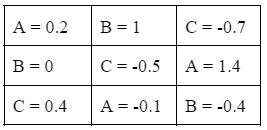
\includegraphics[width=0.5\columnwidth]{Figures/latin square 1.png}
        \caption{Latin Square 1}
        \label{fig:Latin Square 1}
\end{figure}

\begin{figure}[H]
        \centering
    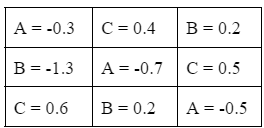
\includegraphics[width=0.5\columnwidth]{Figures/latin square 2.png}
        \caption{Latin Square 2}
        \label{fig:Latin Square 2}
\end{figure}

\begin{figure}[H]
        \centering
    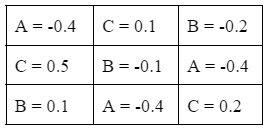
\includegraphics[width=0.5\columnwidth]{Figures/latin square 3.png}
        \caption{Latin Square 3}
        \label{fig:Latin Square 3}
\end{figure}
\newpage
\begin{figure}[H]
        \centering
    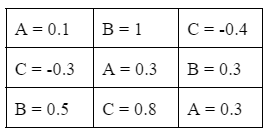
\includegraphics[width=0.5\columnwidth]{Figures/latin square 4.png}
        \caption{Latin Square 4}
        \label{fig:Latin Square 4}
\end{figure}

\begin{figure}[H]
        \centering
    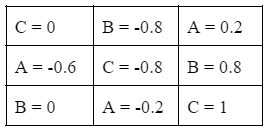
\includegraphics[width=0.5\columnwidth]{Figures/latin square 5.png}
        \caption{Latin Square 5}
        \label{fig:Latin Square 5}
\end{figure}

\begin{figure}[H]
        \centering
    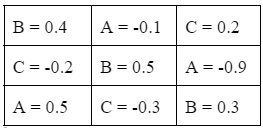
\includegraphics[width=0.5\columnwidth]{Figures/latin square 6.png}
        \caption{Latin Square 6}
        \label{fig:Latin Square 6}
\end{figure}

\begin{figure}[H]
        \centering
    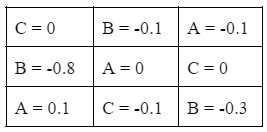
\includegraphics[width=0.5\columnwidth]{Figures/latin square 7.png}
        \caption{Latin Square 7}
        \label{fig:Latin Square 7}
\end{figure}



\end{document}